\section{Hardware}

\subsection{Board}

Board components are annotated in \Fref{fig:board}.  A detailed mechanical drawing describing the board dimensions and locations of key components is available on the \productWebPage{}.

\vskip 2em

\begin{figure}[H]
    \centering
    \begin{tikzpicture}[annotation/.style={circle, draw=black, fill=white, very thick, minimum size=7mm}]
        \node at (0,0) {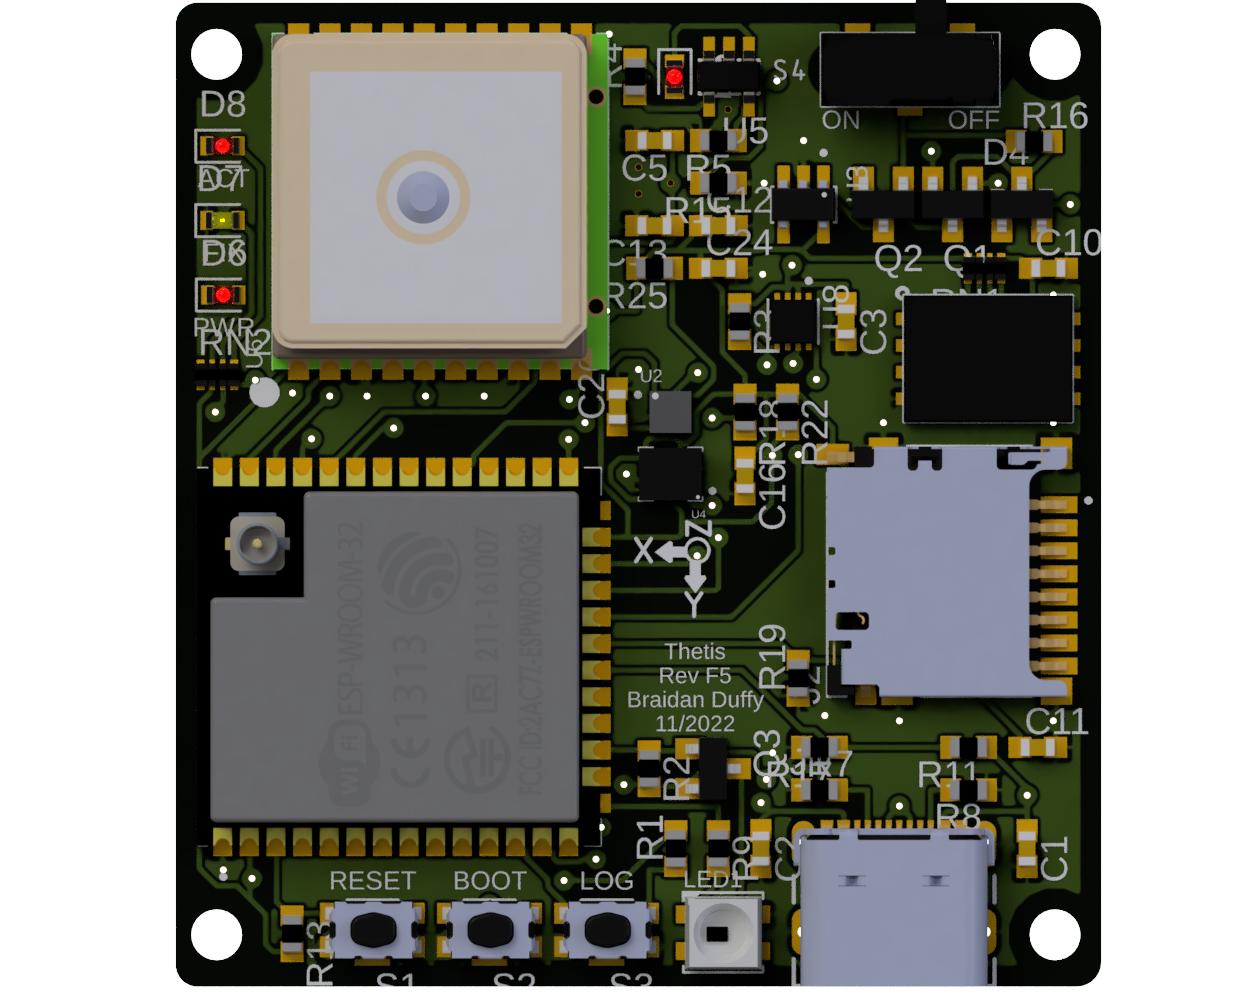
\includegraphics[width=0.95\textwidth]{Images/board.png}};
        \node[annotation] at (-6,-4) {\ref{itm:board1}};
        \node[annotation] at (-6.4,0) {\ref{itm:board2}};
        \node[annotation] at (-5.7,3.7) {\ref{itm:board3}};
        \node[annotation] at (-2.7,1.1) {\ref{itm:board4}};
        \node[annotation] at (4.8,1.8) {\ref{itm:board5}};
        \node[annotation] at (6.0,3.4) {\ref{itm:board6}};
        \node[annotation] at (7.2,3.4) {\ref{itm:board7}};
        \node[annotation] at (6.8,-1.9) {\ref{itm:board8}};
        \node[annotation] at (5.5,-4) {\ref{itm:board9}};
        \node[annotation] at (0.4,-0.8) {\ref{itm:board10}};
        \node[annotation] at (-3.4,-2.9) {\ref{itm:board11}};
    \end{tikzpicture}
    \caption{Board}
    \label{fig:board}
\end{figure}

\vskip 1em

\begin{enumerate}
    \item \label{itm:board1} Power button
    \item \label{itm:board2} \acs{USB}-C connector
    \item \label{itm:board3} \acs{LED}
    \item \label{itm:board4} Serial header
    \item \label{itm:board5} High-g accelerometer
    \item \label{itm:board6} Inertial sensor (gyroscope and accelerometer)
    \item \label{itm:board7} Magnetometer
    \item \label{itm:board8} Wireless antennae
    \item \label{itm:board9} U.FL connector for external wireless antennae
    \item \label{itm:board10} Micro \acs{SD} card socket
    \item \label{itm:board11} Battery connector
\end{enumerate}

\clearpage

\subsection{Housing}

The housing interfaces are annotated in \Fref{fig:housing}.  A detailed mechanical drawing describing the housing dimensions is available on the \productWebPage{}.

\vskip 2em

\begin{figure}[H]
    \centering
    \begin{tikzpicture}[annotation/.style={circle, draw=black, fill=white, very thick, minimum size=7mm}]
        \node at (0,0) {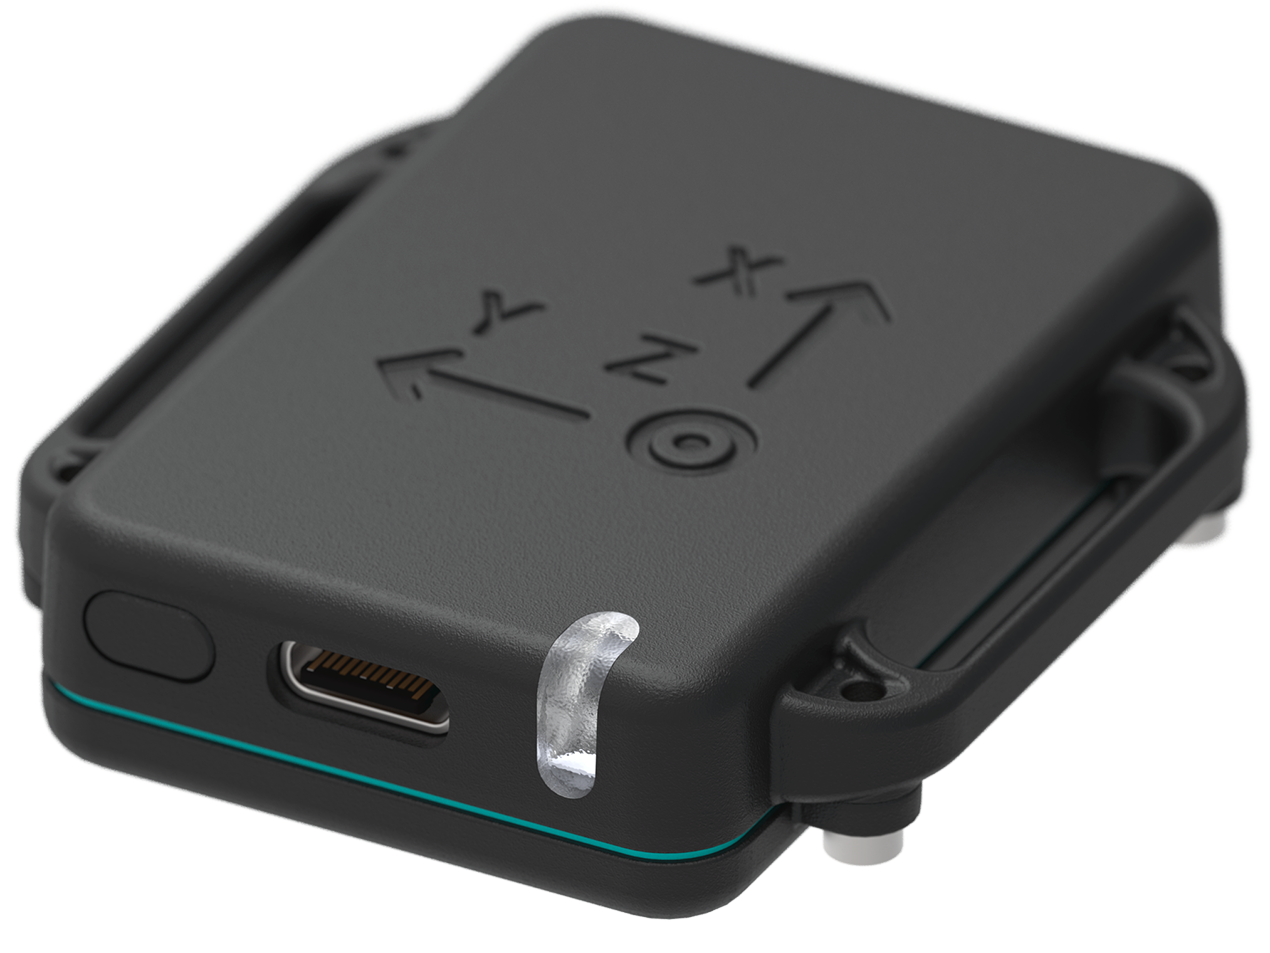
\includegraphics[width=0.8\textwidth]{Images/housing.png}};
        \node[annotation] at (-5.6,-2) {\ref{itm:housing1}};
        \node[annotation] at (-3.7,-2.5) {\ref{itm:housing2}};
        \node[annotation] at (-1.2,-3.2) {\ref{itm:housing3}};
    \end{tikzpicture}
    \caption{Housing}
    \label{fig:housing}
\end{figure}

\vskip 1em

\begin{enumerate}
    \item \label{itm:housing1} Power button
    \item \label{itm:housing2} \acs{USB}-C connector
    \item \label{itm:housing3} \acs{LED}
\end{enumerate}

\clearpage
